\documentclass{article}
\pagenumbering{arabic}
\newcommand{\newCommandName}{text to insert}
% Pages and colors used for the cover page
\usepackage{tikz-page}
\usepackage{url}
\usepackage{lastpage}

% Used for the math and code
\usepackage{amsmath}
\usepackage{listings}
\usepackage{pythonhighlight} % Got this from github! https://github.com/olivierverdier/python-latex-highlighting/blob/master/pythonhighlight.sty

% Used for the pictures
\usepackage{float}
\usepackage{graphicx}

% For the table
\usepackage[utf8]{inputenc}
\usepackage{multirow}
\usepackage{colortbl}

\usepackage[
  top=2cm,
  bottom=2cm,
  left=3cm,
  right=2cm,
  headheight=17pt, % as per the warning by fancyhdr
  includehead,includefoot,
  heightrounded, % to avoid spurious underfull messages
]{geometry} 

% Page numbers/header
\usepackage{fancyhdr}
\definecolor{brickred}{rgb}{0.8, 0.25, 0.33}
\definecolor{cobalt}{rgb}{0.0, 0.28, 0.67}
\definecolor{cadetgrey}{rgb}{0.57, 0.64, 0.69}

% Defining the text box being used for DEPT OF ENG
\tikzset{
        secnode/.style={
                minimum height = .16in,
                minimum width = 4.16in,
                inner xsep = 2pt,
                anchor=north east,
                draw=cadetgrey,
                fill=white,
                text=brickred,
                },
        }


         
\pagestyle{plain}
\renewcommand{\headrulewidth}{0pt}
\begin{document}


% Put name data and assignment number here
\newcommand\personaldate{February 23, 2024}
\newcommand\myname{Leo Berman}
\newcommand\myemail{leo.berman@temple.edu}
\newcommand\hwnum{Exam 1}
\newcommand\mynameabbrev{L. Berman}
\newcommand\assignmenttitle{Exam 1}
\newcommand\yourclass{ECE 8527: Machine Learning and Pattern Recognition}
\begin{titlepage}
	% Drawing the border and the text box 
	\newcommand{\tikzpagelayout}{
		\draw[line width = .04in,
			color = cobalt]
		($(current page.north west)+(1in,-1in)$)
		rectangle ($(current page.south east)+(-.625in,1in)$);

		\draw[line width = .04in,
			color = brickred]
		($(current page.north west)+(.92in,-.92in)$)
		rectangle ($(current page.south east)+(-.705in,1.08in)$);
		\node[secnode] at ($(current page.north west)+(6in,-.875in)$) {\small{\textbf{DEPARTMENT OF ELECTRICAL AND COMPUTER ENGINEERING}}};
	}

	\begin{center}		\break
		\large{\textbf{\assignmenttitle}}\break
		\break
		\large{submitted to \:}\break
		\break
		\large{Professor Joseph Picone}\break
		\large{ECE 8527: Introduction to Pattern Recognition and Machine Learning}\break
		\large{Temple University}\break
		\large{College of Engineering}\break
		\large{1947 North 12th Street}\break
		\large{Philadelphia, Pennsylvania 19122}\break
		\break
		\large{\personaldate}\break
		\break
		\large{prepared by: }\break
		\break
		\large{\myname}\break
		\large{Email: \myemail}
	\end{center}
\end{titlepage}

\newpage
\pagestyle{fancy}
\fancyhead{}
\fancyfoot{}
\fancyhead[R,EH]{Page \thepage\ of \pageref{LastPage}}
\fancyhead[L,EH]{\mynameabbrev: \hwnum}
\fancyfoot[L,EF]{\yourclass}
\fancyfoot[R,EF]{\personaldate}
\renewcommand{\thesection}{\Alph{section}.}
\section{\MakeUppercase{P[E] vs Alpha (Priors Equal)}}
\flushleft{This is the visualization of the data and the visualization of QDA decision surfaces where alpha dictates the position of the bottome left corner of a data set that is 1x1:}
\begin{figure}[!htb]
	\begin{minipage}{0.24\textwidth}
		\centering
		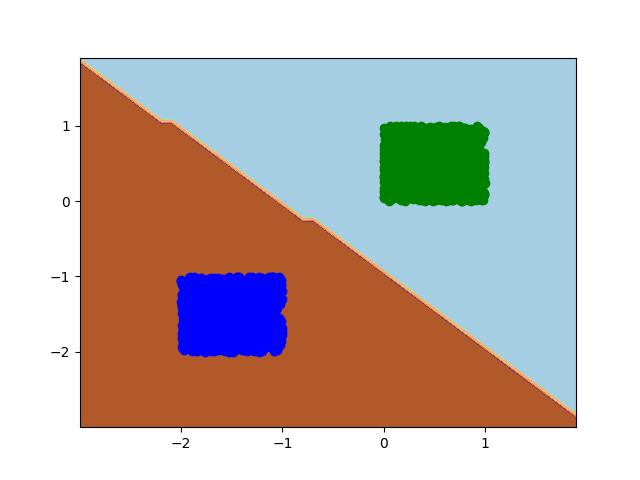
\includegraphics[scale=0.24]{../equalpriors/this0.png};
	\caption{Alpha = -2}
	\end{minipage}
	\begin{minipage}{0.24\textwidth}
			\centering
			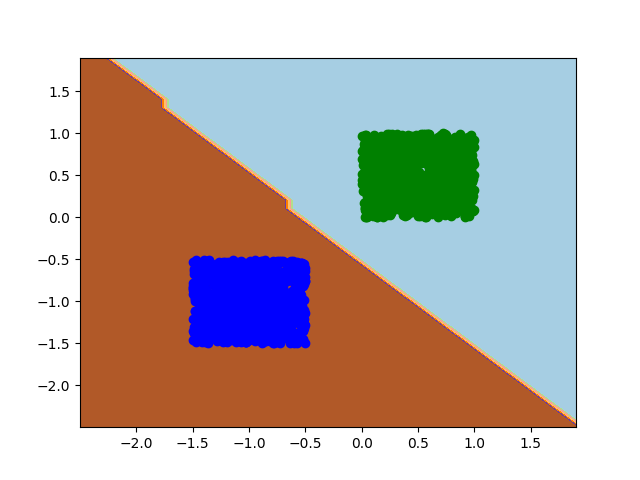
\includegraphics[scale=0.24]{../equalpriors/this4.png}
			\caption{Alpha = -1.42}
	\end{minipage}
	\begin{minipage}{0.24\textwidth}
		\centering
		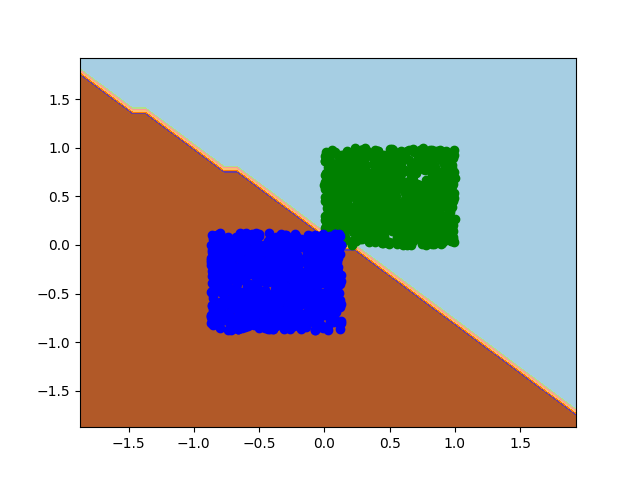
\includegraphics[width=1\linewidth]{../equalpriors/this9.png}
		\caption{Alpha = -0.85}
	\end{minipage}
	\begin{minipage}{0.24\textwidth}
		\centering
		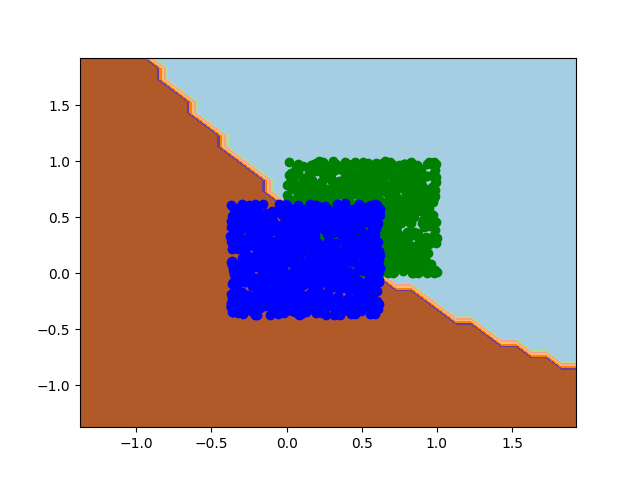
\includegraphics[width=1\linewidth]{../equalpriors/this13.png}
		\caption{Alpha = -0.28}
	\end{minipage}
	\begin{minipage}{0.24\textwidth}
		\centering
		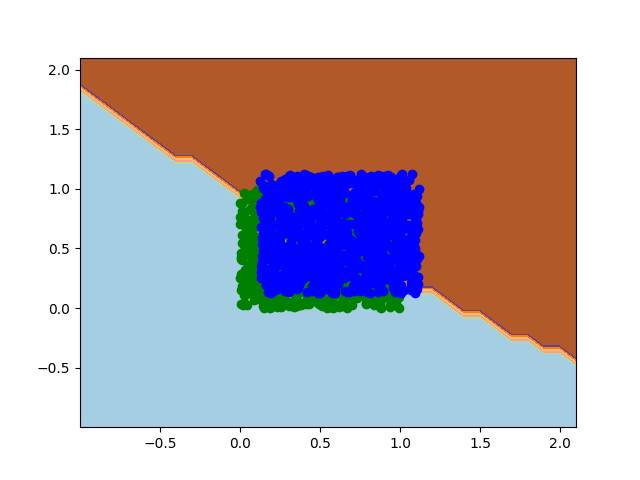
\includegraphics[scale=0.24]{../equalpriors/this17.png};
	\caption{Alpha = 0.28}
	\end{minipage}
	\begin{minipage}{0.24\textwidth}
			\centering
			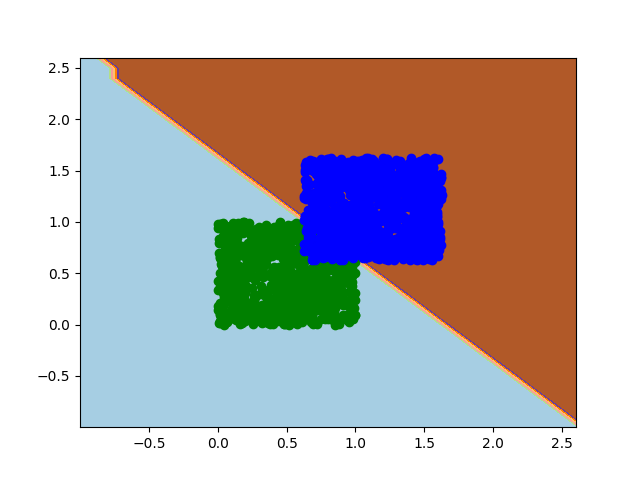
\includegraphics[scale=0.24]{../equalpriors/this21.png}
			\caption{Alpha = 0.85}
	\end{minipage}
	\begin{minipage}{0.24\textwidth}
		\centering
		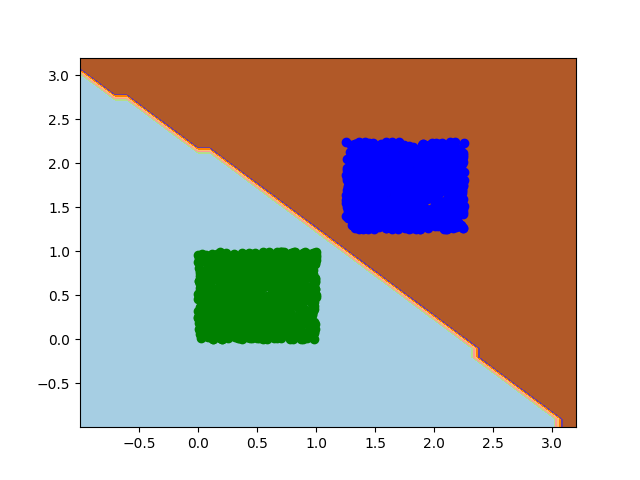
\includegraphics[width=1\linewidth]{../equalpriors/this26.png}
		\caption{Alpha = 1.42}
	\end{minipage}
	\begin{minipage}{0.24\textwidth}
		\centering
		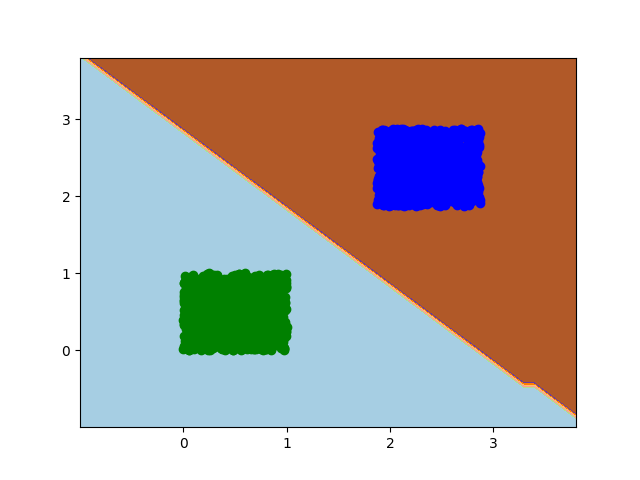
\includegraphics[width=1\linewidth]{../equalpriors/this31.png}
		\caption{Alpha = 2}
	\end{minipage}
\end{figure}
This is the plot of the error rates as a function of alpha.
\begin{figure}[!htb]
	\begin{minipage}{0.99\textwidth}
		\centering
		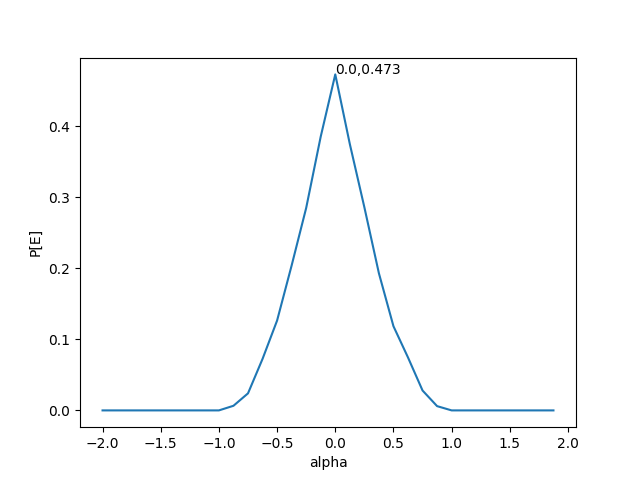
\includegraphics[width=1\linewidth]{../equalpriors/results.png}
		\caption{P[E] vs Alpha (Priors Equal)}
	\end{minipage}
\end{figure}
\clearpage
\section{\MakeUppercase{P[E] vs Alpha (Priors Unequal)}}
\flushleft{This is the visualization of the data and the visualization of QDA decision surfaces where alpha dictates the position of the bottome left corner of a data set that is 1x1:}
\begin{figure}[!htb]
	\begin{minipage}{0.24\textwidth}
		\centering
		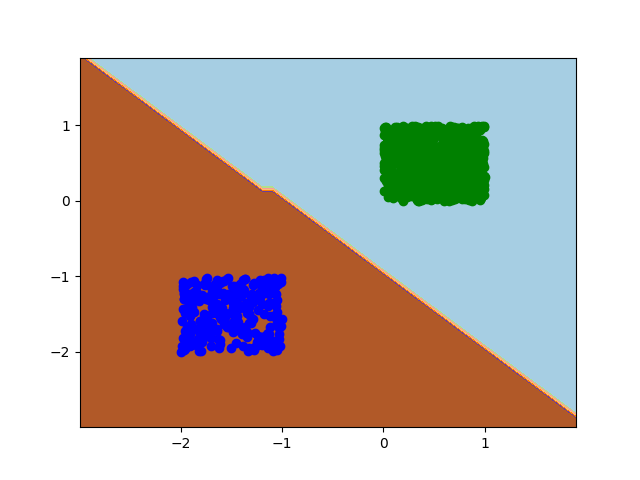
\includegraphics[scale=0.24]{../unequalpriors/this0.png};
	\caption{Alpha = -2}
	\end{minipage}
	\begin{minipage}{0.24\textwidth}
			\centering
			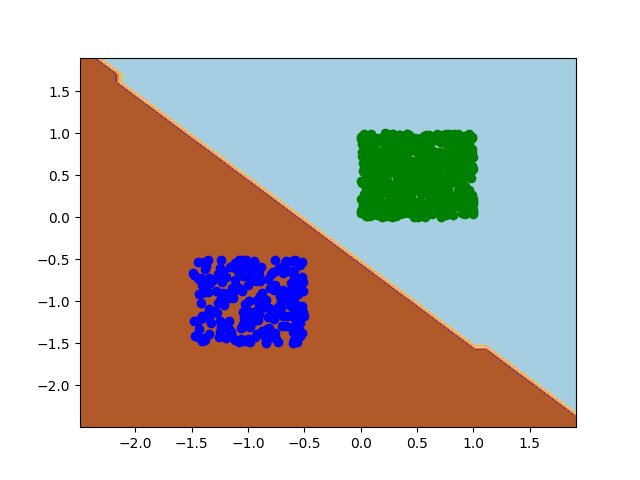
\includegraphics[scale=0.24]{../unequalpriors/this4.png}
			\caption{Alpha = -1.42}
	\end{minipage}
	\begin{minipage}{0.24\textwidth}
		\centering
		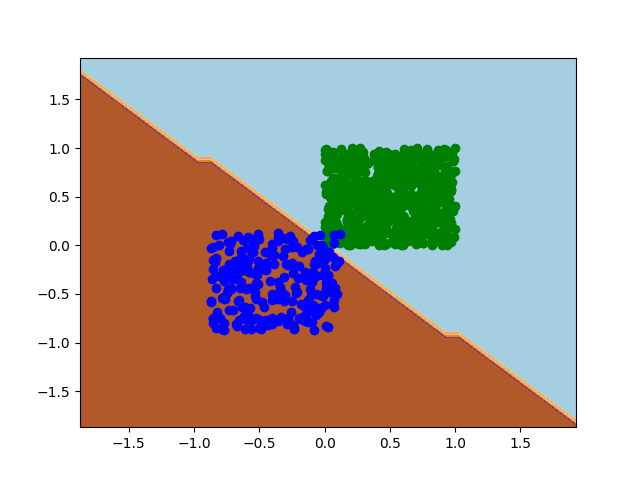
\includegraphics[width=1\linewidth]{../unequalpriors/this9.png}
		\caption{Alpha = -0.85}
	\end{minipage}
	\begin{minipage}{0.24\textwidth}
		\centering
		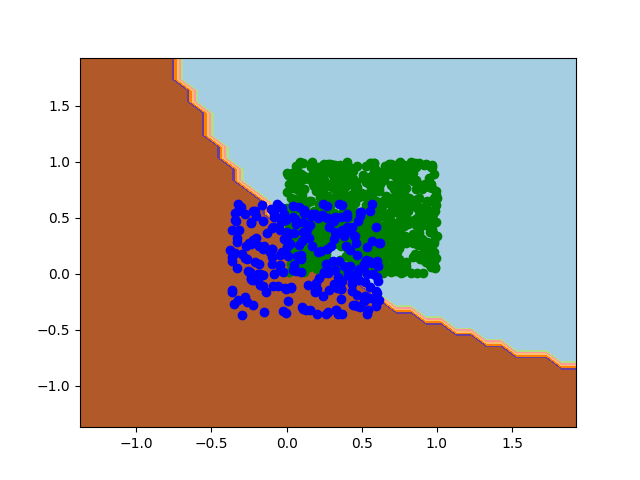
\includegraphics[width=1\linewidth]{../unequalpriors/this13.png}
		\caption{Alpha = -0.28}
	\end{minipage}
	\begin{minipage}{0.24\textwidth}
		\centering
		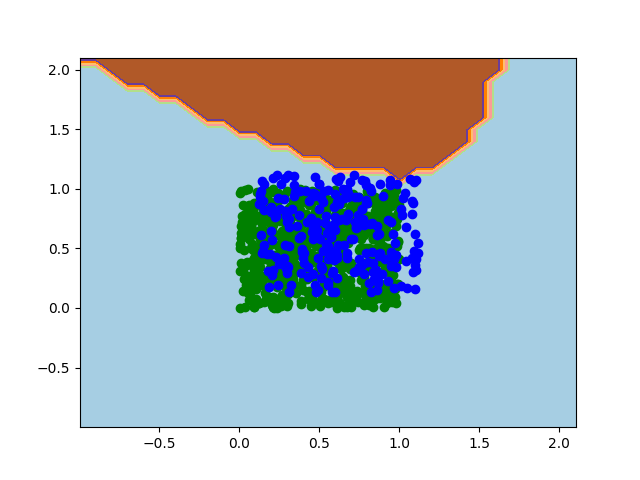
\includegraphics[scale=0.24]{../unequalpriors/this17.png};
	\caption{Alpha = 0.28}
	\end{minipage}
	\begin{minipage}{0.24\textwidth}
			\centering
			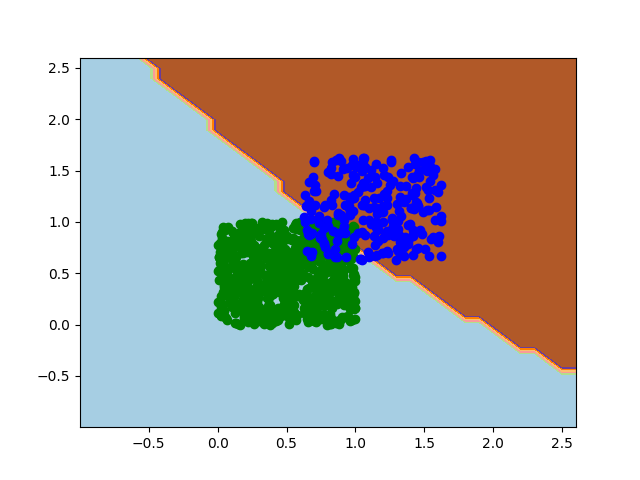
\includegraphics[scale=0.24]{../unequalpriors/this21.png}
			\caption{Alpha = 0.85}
	\end{minipage}
	\begin{minipage}{0.24\textwidth}
		\centering
		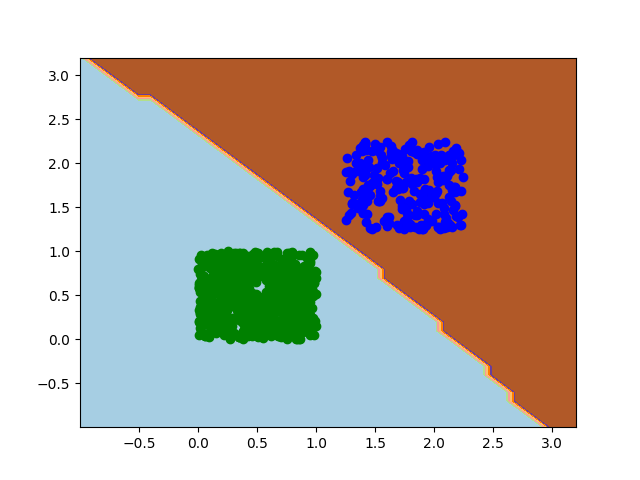
\includegraphics[width=1\linewidth]{../unequalpriors/this26.png}
		\caption{Alpha = 1.42}
	\end{minipage}
	\begin{minipage}{0.24\textwidth}
		\centering
		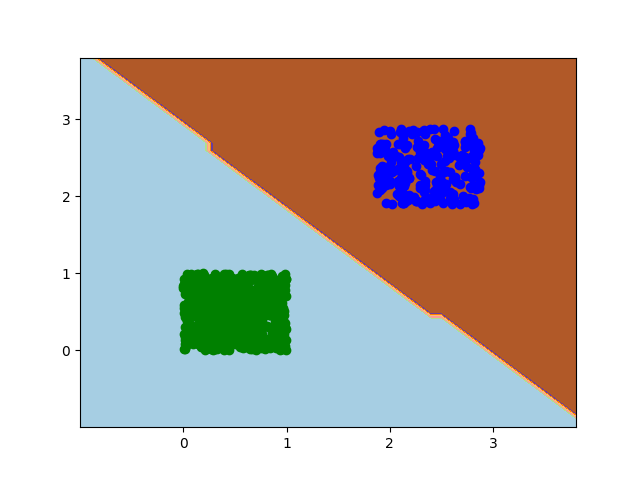
\includegraphics[width=1\linewidth]{../unequalpriors/this31.png}
		\caption{Alpha = 2}
	\end{minipage}
\end{figure}
\flushleft{This is the plot of the error rates as a function of alpha.}
\begin{figure}[!htb]
	\begin{minipage}{0.99\textwidth}
		\centering
		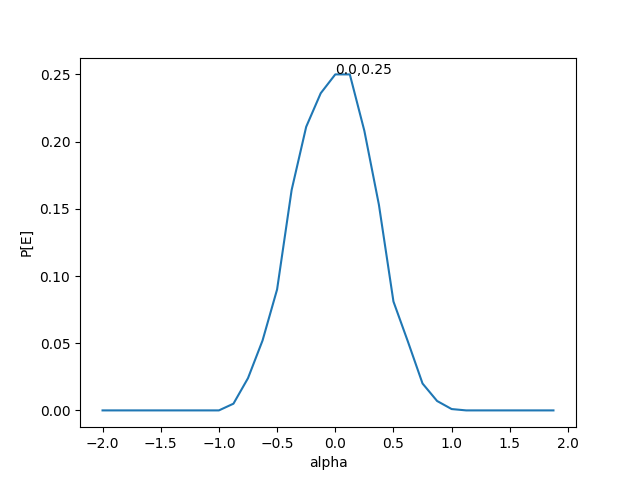
\includegraphics[width=1\linewidth]{../unequalpriors/results.png}
		\caption{P[E] vs. Alpha (Unequal Priors)}
	\end{minipage}
\end{figure}
\clearpage
\pagebreak
\section{\MakeUppercase{Summary}}
\flushleft{When we compare the P[E] as a result of the priors we can see that when scaled, their maximum P[E] correlates to the lowest prior.}
\begin{figure}[!htb]
	\begin{minipage}{0.49\textwidth}
		\centering
		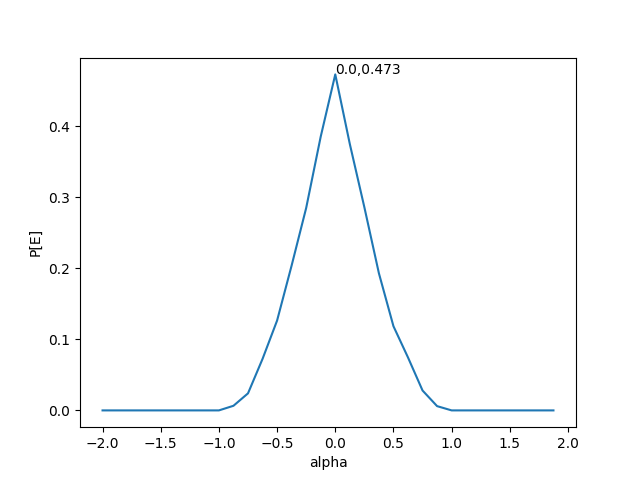
\includegraphics[width=1\linewidth]{../equalpriors/results.png}
		\caption{Equal Priors}
	\end{minipage}
	\begin{minipage}{0.49\textwidth}
		\centering
		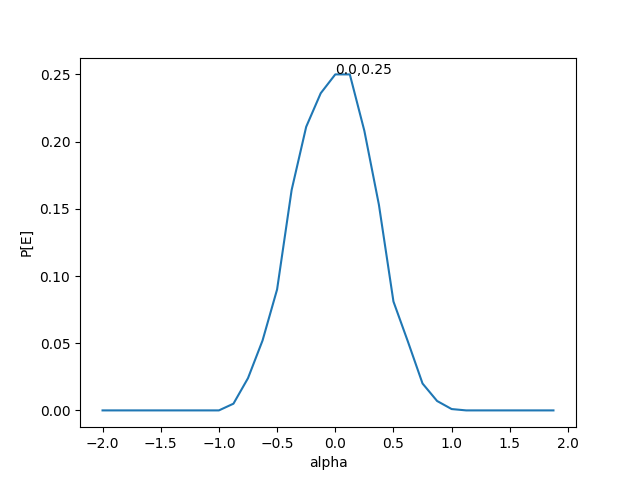
\includegraphics[width=1\linewidth]{../unequalpriors/results.png}
		\caption{Unequal Priors}
	\end{minipage}
\end{figure}

\section{\MakeUppercase{For the diligent student}}
\begin{figure}[!htb]
	\begin{minipage}{0.24\textwidth}
		\centering
		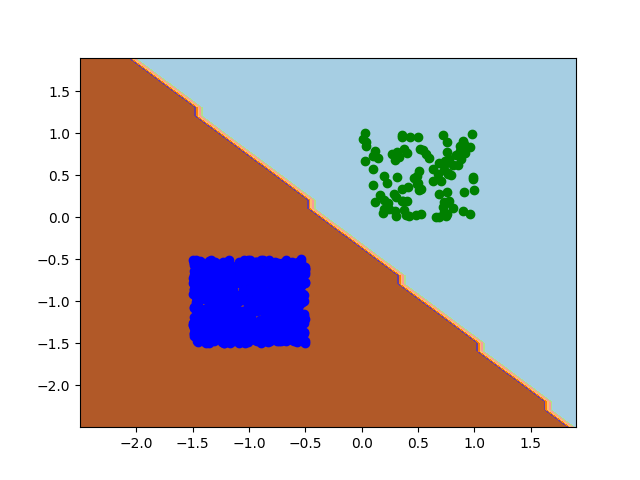
\includegraphics[scale=0.24]{../changingpriors/this0.png};
	\caption{P[w1] = .1, P[w2] = .9}
	\end{minipage}
	\begin{minipage}{0.24\textwidth}
			\centering
			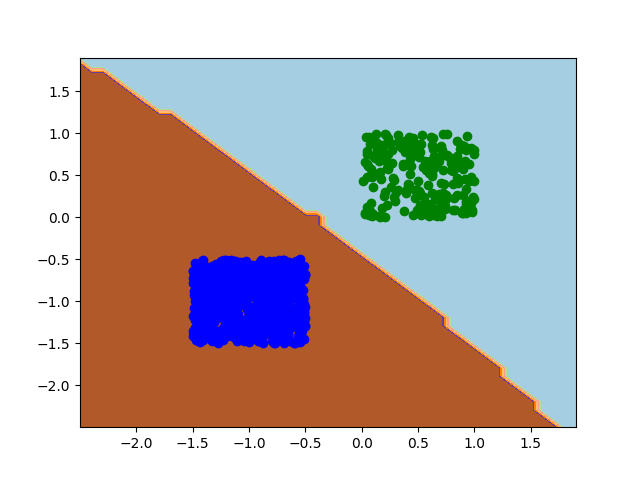
\includegraphics[scale=0.24]{../changingpriors/this4.png}
			\caption{P[w1] = .0.21, P[w2] = .79}
	\end{minipage}
	\begin{minipage}{0.24\textwidth}
		\centering
		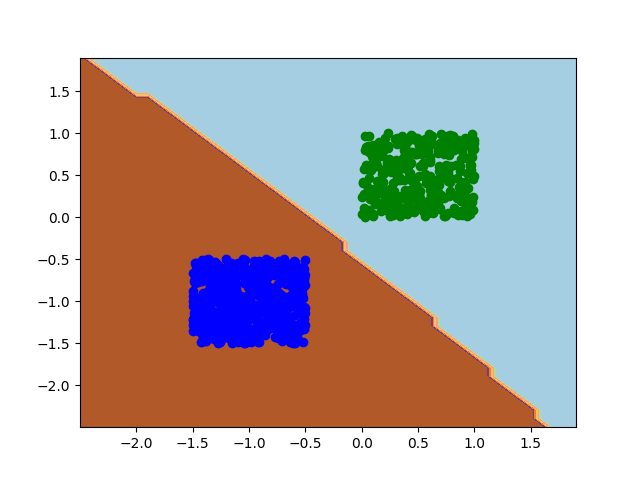
\includegraphics[width=1\linewidth]{../changingpriors/this9.png}
		\caption{P[w1] = .35, P[w2] = .65}
	\end{minipage}
	\begin{minipage}{0.24\textwidth}
		\centering
		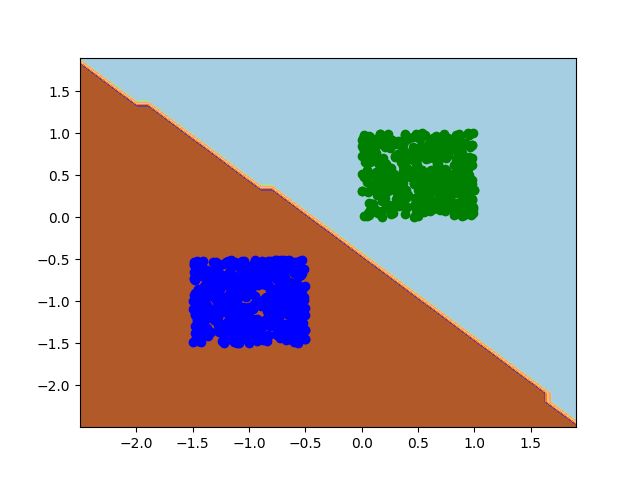
\includegraphics[width=1\linewidth]{../changingpriors/this13.png}
		\caption{P[w1] = .47, P[w2] = .53}
	\end{minipage}
	\begin{minipage}{0.24\textwidth}
		\centering
		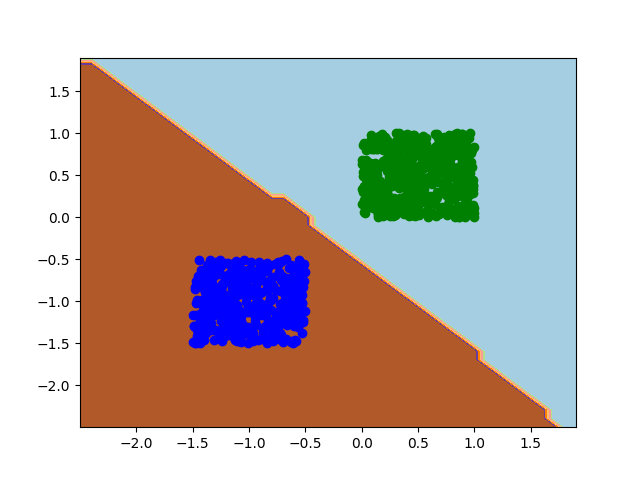
\includegraphics[scale=0.24]{../changingpriors/this17.png};
	\caption{P[w1] = .58, P[w2] = .42}
	\end{minipage}
	\begin{minipage}{0.24\textwidth}
			\centering
			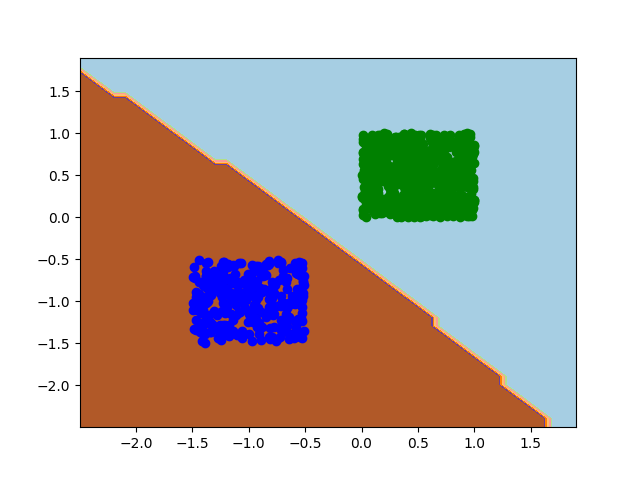
\includegraphics[scale=0.24]{../changingpriors/this21.png}
			\caption{P[w1] = .69, P[w2] = .31}
	\end{minipage}
	\begin{minipage}{0.24\textwidth}
		\centering
		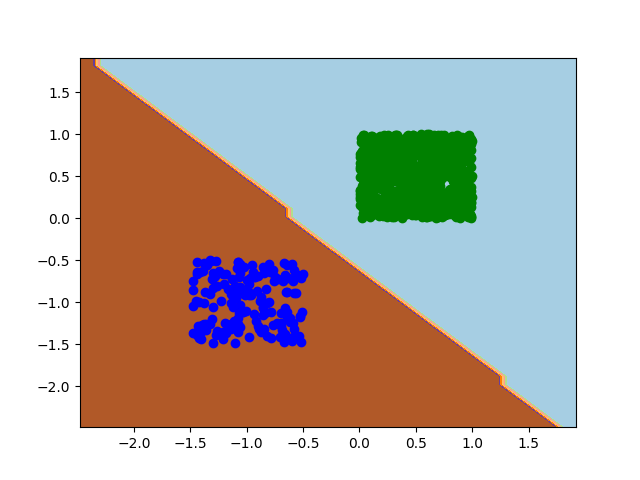
\includegraphics[width=1\linewidth]{../changingpriors/this26.png}
		\caption{P[w1] = .83, P[w2] = .17}
	\end{minipage}
	\begin{minipage}{0.24\textwidth}
		\centering
		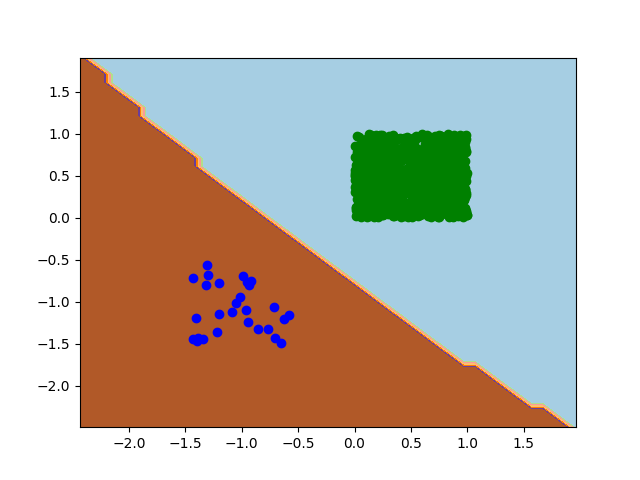
\includegraphics[width=1\linewidth]{../changingpriors/this31.png}
		\caption{P[w1] = .97, P[w2] = .03}
	\end{minipage}
\end{figure}
\flushleft{This is the plot of the error rates as a function of alpha.}
\begin{figure}[!htb]
	\begin{minipage}{0.99\textwidth}
		\centering
		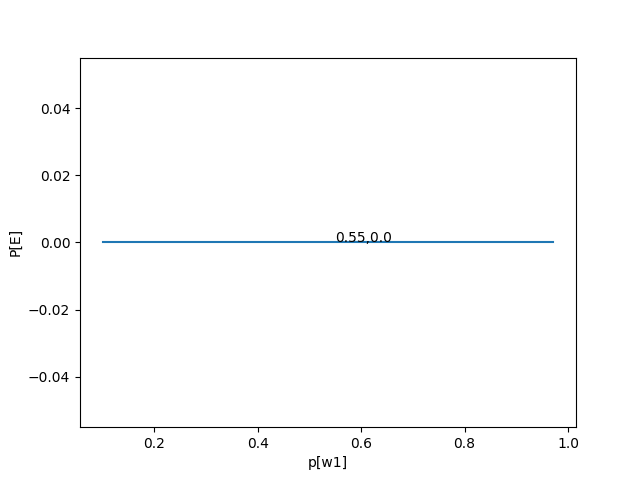
\includegraphics[width=1\linewidth]{../changingpriors/results.png}
		\caption{P[E] vs. Alpha (Unequal Priors)}
	\end{minipage}
\end{figure}
\clearpage
\pagebreak
\section{\MakeUppercase{Appendix}}
Code for Unequal priors:
{
\begin{python}
import numpy as np
import matplotlib.pyplot as plt
import random
from sklearn.decomposition import PCA
from sklearn.multiclass import OneVsRestClassifier
from sklearn.discriminant_analysis import QuadraticDiscriminantAnalysis as QDA
from sklearn.discriminant_analysis import LinearDiscriminantAnalysis as LDA
from sklearn.svm import SVC
from sklearn.inspection import DecisionBoundaryDisplay
import os

# generate data points
def generate_data(x1=0,x2=1,y1=0,y2=1):

	# create lists to store values
	xpoints1 = []
	ypoints1 = []
	xpoints2 = []
	ypoints2 = []
	for i in range(1000):
		xpoints1.append(random.uniform(x1,x2))
		ypoints1.append(random.uniform(x1,x2))
		xpoints2.append(random.uniform(y1,y2))
		ypoints2.append(random.uniform(y1,y2))
	
	# return lists of lists
	return list(map(list, zip(xpoints1, ypoints1))),list(map(list, zip(xpoints2, ypoints2)))

# generate weighted data for second part
def generate_weighted_data(x1=0,x2=1,y1=0,y2=1):

	# create lists to store values
	xpoints1 = []
	ypoints1 = []
	xpoints2 = []
	ypoints2 = []

	# w1        
	for i in range(750):
		xpoints1.append(random.uniform(x1,x2))
		ypoints1.append(random.uniform(x1,x2))

	#w2
	for i in range(250):
		xpoints2.append(random.uniform(y1,y2))
		ypoints2.append(random.uniform(y1,y2))
	
	# return lists of lists
	return list(map(list, zip(xpoints1, ypoints1))),list(map(list, zip(xpoints2, ypoints2)))

# plot the decision surfaces
def plot_qda_decision_surfaces(data1,qda):

	# calculate the bounds of the data set
	min1, max1 = data1[:, 0].min()-1, data1[:,  0].max()+1
	min2, max2 = data1[:, 1].min()-1, data1[:, 1].max()+1

	# arrange the data sets so they are evenly spaced
	x1grid = np.arange(min1, max1, 0.1)
	x2grid = np.arange(min2, max2, 0.1)

	# create a meshgrid
	xx, yy = np.meshgrid(x1grid, x2grid)

	# flatten the grid
	r1, r2 = xx.flatten(), yy.flatten()

	# reshape them into vectors of the right size
	r1, r2 = r1.reshape((len(r1), 1)), r2.reshape((len(r2), 1))
	
	# concatenate the vectors
	grid = np.hstack((r1,r2))

	# create a prediction for all the values
	yhat = qda.predict(grid)

	# reshape the x value to be an axis
	zz = yhat.reshape(xx.shape)

	# contour the plots with paried colors
	plt.contourf(xx, yy, zz, cmap='Paired')
		
# plot lda decision surface
def plot_lda_decision_surfaces(data1,lda):

	# calculate intercept and coefficients
	b, w1, w2 = lda.intercept_[0], lda.coef_[0][0], lda.coef_[0][1]    

	# calculate the line
	x1 = np.array([np.min(data1[:,0], axis=0), np.max(data1[:,0], axis=0)])
	y1 = -(b+x1*w1)/w2

	# plot the line
	plt.plot(x1,y1,c="r")
	

def main():
	
		# lists for probability of error
		probability_error = []
	
		# list for xaxis
		xaxis = []
	
		# resolution
		iterations = 40
	
		# remove frames from previous
		os.system("rm this*.png")
	
		# iterate through the resolutions
		for i in range(iterations):
	
			# generate the data
			data1,data2 = generate_weighted_data(0,1,-2+(i/(iterations/4)),-1+(i/(iterations/4)))
	
			# generate the labels
			labels = [0]*len(data1) + [1]*len(data2)
	
			# copy the lists for later testing
			test1 = data1.copy()
			test2 = data2.copy()
	
			# concatenate data
			data1.extend(data2)
			data1 = np.array(data1)
	
			# create a QDA model
			model = QDA()
	
			# fit model to the data
			model.fit(data1,labels)
	
			# set the priors
			model.priors=[.75,.25]
	
			# calculate the probability of error
			probability_error.append(1-model.score(data1,labels))
	
			# append to the axis
			xaxis.append(-2 + i/(iterations/4))
	
			# create lists for each x and y for each data set
			# for plotting the scatter
			xes1 = []
			yes1 = []
			xes2 = []
			yes2 = []
			for x in range(len(test1)):
				xes1.append(test1[x][0])
				yes1.append(test1[x][1])
			for x in range(len(test2)):
				xes2.append(test2[x][0])
				yes2.append(test2[x][1])
			
			# plot the lda decision surfaces
			# plot_lda_decision_surfaces(data1,model)
			
			#plot the qda decision surfaces
			plot_qda_decision_surfaces(data1,model)
	
			# plot the two datasets
			plt.scatter(xes1,yes1,color = "green")
			plt.scatter(xes2,yes2,color = "blue")
	
			# save the plots as images
			plt.savefig("this"+str(i)+".png")
	
			# clear plots
			plt.cla()
		
		# plot the probability of errors
		plt.plot(xaxis,probability_error)
	
		# label axis
		plt.xlabel("alpha")
		plt.ylabel("P[E]")
	
		# label the middle point
		plt.text(xaxis[iterations//2],probability_error[iterations//2],str(xaxis[iterations//2]) + "," + str(probability_error[iterations//2]))
		
		# save this image
		plt.savefig("results.png")
	
	
	main()
	
	
	
\end{python}

Code for the equal priors
\begin{python}
import numpy as np
import matplotlib.pyplot as plt
import random
from sklearn.decomposition import PCA
from sklearn.multiclass import OneVsRestClassifier
from sklearn.discriminant_analysis import QuadraticDiscriminantAnalysis as QDA
from sklearn.discriminant_analysis import LinearDiscriminantAnalysis as LDA
from sklearn.svm import SVC
from sklearn.inspection import DecisionBoundaryDisplay
import os

# generate data points
def generate_data(x1=0,x2=1,y1=0,y2=1):

	# create lists to store values
	xpoints1 = []
	ypoints1 = []
	xpoints2 = []
	ypoints2 = []
	for i in range(1000):
		xpoints1.append(random.uniform(x1,x2))
		ypoints1.append(random.uniform(x1,x2))
		xpoints2.append(random.uniform(y1,y2))
		ypoints2.append(random.uniform(y1,y2))
	
	# return lists of lists
	return list(map(list, zip(xpoints1, ypoints1))),list(map(list, zip(xpoints2, ypoints2)))

# generate weighted data for second part
def generate_weighted_data(x1=0,x2=1,y1=0,y2=1):

	# create lists to store values
	xpoints1 = []
	ypoints1 = []
	xpoints2 = []
	ypoints2 = []

	# w1        
	for i in range(750):
		xpoints1.append(random.uniform(x1,x2))
		ypoints1.append(random.uniform(x1,x2))

	#w2
	for i in range(250):
		xpoints2.append(random.uniform(y1,y2))
		ypoints2.append(random.uniform(y1,y2))
	
	# return lists of lists
	return list(map(list, zip(xpoints1, ypoints1))),list(map(list, zip(xpoints2, ypoints2)))

# plot the decision surfaces
def plot_qda_decision_surfaces(data1,qda):

	# calculate the bounds of the data set
	min1, max1 = data1[:, 0].min()-1, data1[:,  0].max()+1
	min2, max2 = data1[:, 1].min()-1, data1[:, 1].max()+1

	# arrange the data sets so they are evenly spaced
	x1grid = np.arange(min1, max1, 0.1)
	x2grid = np.arange(min2, max2, 0.1)

	# create a meshgrid
	xx, yy = np.meshgrid(x1grid, x2grid)

	# flatten the grid
	r1, r2 = xx.flatten(), yy.flatten()

	# reshape them into vectors of the right size
	r1, r2 = r1.reshape((len(r1), 1)), r2.reshape((len(r2), 1))
	
	# concatenate the vectors
	grid = np.hstack((r1,r2))

	# create a prediction for all the values
	yhat = qda.predict(grid)

	# reshape the x value to be an axis
	zz = yhat.reshape(xx.shape)

	# contour the plots with paried colors
	plt.contourf(xx, yy, zz, cmap='Paired')
		
# plot lda decision surface
def plot_lda_decision_surfaces(data1,lda):

	# calculate intercept and coefficients
	b, w1, w2 = lda.intercept_[0], lda.coef_[0][0], lda.coef_[0][1]    

	# calculate the line
	x1 = np.array([np.min(data1[:,0], axis=0), np.max(data1[:,0], axis=0)])
	y1 = -(b+x1*w1)/w2

	# plot the line
	plt.plot(x1,y1,c="r")
	

def main():

	# lists for probability of error
	probability_error = []

	# list for xaxis
	xaxis = []

	# resolution
	iterations = 32

	# remove frames from previous
	os.system("rm this*.png")

	# iterate through the resolutions
	for i in range(iterations):

		# generate the data
		data1,data2 = generate_data(0,1,-2+(i/(iterations/4)),-1+(i/(iterations/4)))

		# generate the labels
		labels = [0]*len(data1) + [1]*len(data2)

		# copy the lists for later testing
		test1 = data1.copy()
		test2 = data2.copy()

		# concatenate data
		data1.extend(data2)
		data1 = np.array(data1)

		# create a QDA model
		model = QDA()

		# fit model to the data
		model.fit(data1,labels)

		# set the priors
		model.priors=[.5,.5]

		# calculate the probability of error
		probability_error.append(1-model.score(data1,labels))

		# append to the axis
		xaxis.append(-2 + i/(iterations/4))

		# create lists for each x and y for each data set
		# for plotting the scatter
		xes1 = []
		yes1 = []
		xes2 = []
		yes2 = []
		for x in range(len(test1)):
			xes1.append(test1[x][0])
			yes1.append(test1[x][1])
		for x in range(len(test2)):
			xes2.append(test2[x][0])
			yes2.append(test2[x][1])
		
		# plot the lda decision surfaces
		# plot_lda_decision_surfaces(data1,model)
		
		#plot the qda decision surfaces
		plot_qda_decision_surfaces(data1,model)

		# plot the two datasets
		plt.scatter(xes1,yes1,color = "green")
		plt.scatter(xes2,yes2,color = "blue")

		# save the plots as images
		plt.savefig("this"+str(i)+".png")

		# clear plots
		plt.cla()
	
	# plot the probability of errors
	plt.plot(xaxis,probability_error)

	# label axis
	plt.xlabel("alpha")
	plt.ylabel("P[E]")

	# label the middle point
	plt.text(xaxis[iterations//2],probability_error[iterations//2],str(xaxis[iterations//2]) + "," + str(probability_error[iterations//2]))
	
	# save this image
	plt.savefig("results.png")


main()

	
	
\end{python}
}
\end{document}